\documentclass{beamer}
\usepackage[utf8]{inputenc}
\usepackage[frenchb]{babel}
\usepackage[T1]{fontenc}
\usepackage{graphics}
\usepackage{framed}
\usepackage{graphicx}
\usepackage{grffile}
\usepackage{longtable}
\usepackage{wrapfig}
\usepackage{rotating}
\usepackage[normalem]{ulem}
\usepackage{amsmath}
\usepackage{textcomp}
\usepackage{amssymb}
\usepackage{capt-of}
\usetheme{Warsaw}

\title[Support pour Verificarlo]{Support de MPI/OpenMP et de la vectorisation dans Verificarlo}
\subtitle{Master Calcul Haute Performance et Simulation}

\author[Hery, Ali, Nicolas]{Hery ANDRIANANTENAINA \\ Ali LAKBAL \\ Nicolas BOUTON}

\institute{\textbf{Encadrant:} Eric PETIT}

\date{Année 2020-2021}

\begin{document}

\maketitle

\begin{frame}{Verificarlo}

  \begin{itemize}
  \item Compilateur: \textbf{ Clang et llvm} 
  \item Domaine d'utilisation: \textbf{ Instrumentation des opérations flottantes}
  \end{itemize}
  
  \textbf{1. Vectorisation dans le calcul scientifique}
  
\end{frame}

\begin{frame}{Changements aux niveaux des backends}

  \begin{block}{Fonctions vectorielles en mode scalaire}
    Tous les backends
  \end{block}

  \begin{block}{Fonctions vectorielles en mode vectoriel}
    \begin{itemize}
    \item ieee
    \item vprec
    \end{itemize}
  \end{block}

\end{frame}

\begin{frame}{Changements aux niveaux du backend vprec}

  \begin{block}{Fonctionnement du backend}
    \begin{itemize}
    \item norme IEEE754
    \item fonction de debug
    \end{itemize}
  \end{block}

  \begin{block}{Opérande constantes}
    \begin{itemize}
    \item avertissement de clang sur les types des paramètres de fonction
    \item ajout d'un pragma pour retirer l'avertissement
    \end{itemize}
  \end{block}

\end{frame}

\begin{frame}{Changements aux niveaux du backend vprec}

  \begin{block}{Fonctionnement du backend}
    \begin{itemize}
    \item nombres fini et infini
    \item nombres normaux et dénormaux
    \end{itemize}
  \end{block}

  \begin{figure}
    \centering
    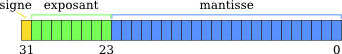
\includegraphics[width=200px]{../ressources/IEEE754_simple_precision.png}
    \caption{\label{fig:ieee_simple_precision}Représentation d'un nombre flottant simple précision}
  \end{figure}

\end{frame}

\begin{frame}{Compilation}

  \begin{block}{Ajout dans verificarlo}
    Compilation des \textbf{wrappers} et des \textbf{backends} avec le drapeau
    \textbf{-march=native}
  \end{block}

\end{frame}

\begin{frame}{Problèmes rencontrés}

  \begin{block}{Types vectorielles}
    Vecteur de 4 double précision
  \end{block}

  \begin{block}{Jeu d'instruction disponnible}
    SSE
  \end{block}

  \begin{block}{Clang}
    Utilise 4 addition vectoriel SSE
  \end{block}

  \begin{block}{Verificarlo}
    \begin{itemize}
    \item Backend: vectorisé comme pour clang
    \item Problème: vecteur passé par registre entre les modules
    \end{itemize}
  \end{block}

\end{frame}

\begin{frame}{Conclusion}

  \begin{block}{Cours en relation}
    Architecture Parallèle
  \end{block}

\end{frame}

\end{document}
